%% Based on a TeXnicCenter-Template by Gyorgy SZEIDL.
%%%%%%%%%%%%%%%%%%%%%%%%%%%%%%%%%%%%%%%%%%%%%%%%%%%%%%%%%%%%%

%------------------------------------------------------------
%
\documentclass{article}%
%Options -- Point size:  10pt (default), 11pt, 12pt
%        -- Paper size:  letterpaper (default), a4paper, a5paper, b5paper
%                        legalpaper, executivepaper
%        -- Orientation  (portrait is the default)
%                        landscape
%        -- Print size:  oneside (default), twoside
%        -- Quality      final(default), draft
%        -- Title page   notitlepage, titlepage(default)
%        -- Columns      onecolumn(default), twocolumn
%        -- Equation numbering (equation numbers on the right is the default)
%                        leqno
%        -- Displayed equations (centered is the default)
%                        fleqn (equations start at the same distance from the right side)
%        -- Open bibliography style (closed is the default)
%                        openbib
% For instance the command
%           \documentclass[a4paper,12pt,leqno]{article}
% ensures that the paper size is a4, the fonts are typeset at the size 12p
% and the equation numbers are on the left side
%
\usepackage{amsmath}%
\usepackage{amsfonts}%
\usepackage{amssymb}%
\usepackage{graphicx}
%-------------------------------------------
\newtheorem{theorem}{Theorem}
\newtheorem{acknowledgement}[theorem]{Acknowledgement}
\newtheorem{algorithm}[theorem]{Algorithm}
\newtheorem{axiom}[theorem]{Axiom}
\newtheorem{case}[theorem]{Case}
\newtheorem{claim}[theorem]{Claim}
\newtheorem{conclusion}[theorem]{Conclusion}
\newtheorem{condition}[theorem]{Condition}
\newtheorem{conjecture}[theorem]{Conjecture}
\newtheorem{corollary}[theorem]{Corollary}
\newtheorem{criterion}[theorem]{Criterion}
\newtheorem{definition}[theorem]{Definition}
\newtheorem{example}[theorem]{Example}
\newtheorem{exercise}[theorem]{Exercise}
\newtheorem{lemma}[theorem]{Lemma}
\newtheorem{notation}[theorem]{Notation}
\newtheorem{problem}[theorem]{Problem}
\newtheorem{proposition}[theorem]{Proposition}
\newtheorem{remark}[theorem]{Remark}
\newtheorem{solution}[theorem]{Solution}
\newtheorem{summary}[theorem]{Summary}
\newenvironment{proof}[1][Proof]{\textbf{#1.} }{\ \rule{0.5em}{0.5em}}

\begin{document}

\begin{flushleft}
\textbf{Course:} CSC707, Automata, Computability and Computational Theory\\
\textbf{Homework 6}: Context-free languages, context-free grammars, PDA, Pumping lemma. \\
\textbf{Submission:} Use Wolfware\\
\textbf{File Format:} LaTeX and PDF, and any images you have\\
\end{flushleft}

\begin{center}
\fbox{\textbf{Due Date:} \textbf{2:00 A.M. (EST), Tuesday, April 13, 2010}}\\
\end{center}

\noindent{\hrulefill}

\bigskip

\begin{enumerate}

	\item Prove non-context-free using Pumping lemma:
	\begin{enumerate}
		\item $ L = \{ 0^i 1^j 2^i 3^j |i,j \ge 1\} $
		\item $ L = \{ a^i b^j c^k |0 \le i < j < k\} $
		\item $ L = \{ a^i b^j |j = i^2 \} $
		\item $ {\bar L}$, where $L = \{ 0^k |k$  is a perfect square $\}$
	\end{enumerate}
	
  
\begin{enumerate}
	\item 
	\begin{theorem}
	$ L = \{ 0^i 1^j 2^i 3^j |i,j \ge 1\} $ is non-context-free.
	\end{theorem}
	\begin{proof}
	We can use pumping lemma to prove it.
	
  1. For $\forall p$, we choose $s = 0^p 1^p 2^p 3^p \in L \bigcap \Sigma ^{\geq p}$. 
  
  2. $\forall u,v,x,y,z, s = uvxyz, s.t. |vy| \geq 1$ and $|vxy| \leq p$.
  
  3. Choose $i = 2$, we need to prove $s = uv^2xy^2z \notin L$.
  
  4. Consider all the cases of $v$ and $y$:
  
\begin{itemize}
	\item Case 1: Both $v$ and $y$ contain only a same number: \\
	
	$\frac{v}{y} | \frac{0^m}{0^n}| \frac{1^m}{1^n}| \frac{2^m}{2^n}| \frac{3^m}{3^n}$\\
	
	When $i = 2$, the number of 0 (or 1,2,3) would be $p+m+n$. By (2), $m+n \geq 1 \Rightarrow p+m+n \neq p$. Thus $s = uv^2xy^2z \notin L$. \\
	
	\item Case 2: Both $v$ and $y$ contain one number but they are different and $m \geq 1, n \geq 1$: \\
	
	$\frac{v}{y} | \frac{0^m}{1^n}| \frac{1^m}{2^n}| \frac{2^m}{3^n}$\\
	
	When $i = 2$, the number of 0 and 1 (or 1 and 2, 2 and 3) would be $p+m$ and $p+n$, respectively. Since $p+m \neq p $ and $p+n \neq p$, $s = uv^2xy^2z \notin L$.\\
	
	\item Case 3: Either $v$ or $y$ contain two numbers and $m \geq 1, n \geq 1, k \geq 1$: \\
	
	$\frac{v}{y} | \frac{0^m1^k}{1^n}| \frac{0^m}{0^n1^k}| \frac{1^m2^k}{2^n}| \frac{1^m}{1^n2^k}| \frac{2^m 1^k}{3^n}| \frac{2^m}{2^n3^k}$\\
	
	When $i = 2$, $s$ will have interleaving patterns, such as $0^m1^k0^m1^k$. Thus $s = uv^2xy^2z \notin L$.
	
	
\end{itemize}
5. 	$ L = \{ 0^i 1^j 2^i 3^j |i,j \ge 1\} $ is non-context-free.
	\end{proof}
	
			\item 
	\begin{theorem}
$ L = \{ a^i b^j c^k |0 \le i < j < k\} $
	\end{theorem}
	\begin{proof}
	We can use pumping lemma to prove it.
	
  1. For $\forall p$, we choose $s = a^p b^{p+1} c^{p+2} \in L \bigcap \Sigma ^{\geq p}$. 
  
  2. $\forall u,v,x,y,z, s = uvxyz, s.t. |vy| \geq 1$ and $|vxy| \leq p$.
  
  3. Consider all the cases of $v$ and $y$:
  
\begin{itemize}
	\item Case 1: Both $v$ and $y$ contain only a same number: \\
	
	$\frac{v}{y} | \frac{a^m}{a^n}| \frac{b^m}{b^n}| \frac{c^m}{c^n}$\\
	
	For $v = a , y = a$, we choose $i = 2$. In this way, the number of $a$ would be $p+m+n$. By (2), $m+n \geq 1 \Rightarrow p+m+n \geq p + 1$. Thus $s = uv^2xy^2z = a^{p+m+n}b^{p+1}c^{p+2} \notin L$. \\
	
  For $v = b , y = b$, we choose $i = 2$. In this way, the number of $b$ would be $p+m+n$. By (2), $m+n \geq 1 \Rightarrow p+1m+n \geq p + 2$. Thus $s = uv^2xy^2z = a^{p}b^{p+m+n+1}c^{p+2} \notin L$. \\
		
	For $v = c , y = c$, we choose $i = 0$. In this way, the number of $c$ would be $p-m-n$. By (2), $m+n \geq 1 \Rightarrow p+2-(m+n) \leq p + 1$. Thus $s = uv^2xy^2z = a^{p}b^{p+1}c^{p+2-(m+n)} \notin L$. \\
	
	\item Case 2: Both $v$ and $y$ contain one number but they are different and $m \geq 1, n \geq 1$: \\
	
	$\frac{v}{y} | \frac{a^m}{b^n}| \frac{b^m}{c^n}$\\
	
	For $v = a , y = b$, we choose $i = 2$. In this way, the number of $b$ would be $p - n$. $p+1+n \geq p + 2$. Thus $s = uv^2xy^2z = a^{p+m}b^{p+1_n}c^{p+2} \notin L$. \\
	
	For $v = b , y = c$, we choose $i = 0$. In this way, the number of $b$ would be $p + 1 - n$. $p+1-m \leq p$. Thus $s = uv^2xy^2z = a^{p}b^{p+1-m}c^{p+2-n} \notin L$. \\
	
	\item Case 3: Either $v$ or $y$ contain two numbers and $m \geq 1, n \geq 1, k \geq 1$: \\
	 
	$\frac{v}{y} | \frac{a^mb^k}{b^n}| \frac{a^m}{a^nb^k}| \frac{b^mc^k}{c^n}| \frac{b^m}{b^nc^k}$\\
	
	When $i = 2$, $s$ will have interleaving patterns, such as $a^mb^ka^mb^k$. Thus $s = uv^2xy^2z \notin L$.
	
	
\end{itemize}
5. 	$ L = \{ 0^i 1^j 2^i 3^j |i,j \ge 1\} $ is non-context-free.
	\end{proof}
	
		\item 
	\begin{theorem}
$ L = \{ a^i b^j |j = i^2 \} $
	\end{theorem}
	\begin{proof}
	
	We can use pumping lemma to prove it.
	
  1. For $\forall p$, we choose $s = a^p b^{p^2}  \in L \bigcap \Sigma ^{\geq p}$. 
  
  2. $\forall u,v,x,y,z, s = uvxyz, s.t. |vy| \geq 1$ and $|vxy| \leq p$.
  
  3. Consider all the cases of $v$ and $y$:
  
\begin{itemize}
	\item Case 1: Both $v$ and $y$ contain only a same number: \\
	
	$\frac{v}{y} | \frac{a^m}{a^n}| \frac{b^m}{b^n}$\\
	
	For $v = a , y = a$, we choose $i = 2$. In this way, the number of $a$ would be $p+m+n$. By (2), $m+n \geq 1 \Rightarrow (p+m+n)^2 \neq p^2$. Thus $s = uv^2xy^2z = a^{p+m+n}b^{p^2} \notin L$. \\
	
  For $v = b , y = b$, we choose $i = 2$. In this way, the number of $b$ would be $p^2+m+n$. By (2), $m+n \geq 1 \Rightarrow p^2+m+n \neq p^2$. Thus $s = uv^2xy^2z = a^{p}b^{p^2+m+n} \notin L$. \\
		
	
	\item Case 2: Both $v$ and $y$ contain one number but they are different and $m \geq 1, n \geq 1$: \\
	
	$\frac{v}{y} | \frac{a^m}{b^n}$\\
	
	For $v = a , y = b$, we choose $i = 2$. In this way, the number of $a$ would be $p + m$ and the number of $b$ would be $p^2 + n$. Since $(p + m)^2 = p^2 + 2mp + m^2 > p^2 + n$. Thus $s = uv^2xy^2z = a^{p+m}b^{p^2+n} \notin L$. \\
	
	\item Case 3: Either $v$ or $y$ contain two numbers and $m \geq 1, n \geq 1, k \geq 1$: \\
	 
	$\frac{v}{y} | \frac{a^mb^k}{b^n}| \frac{a^m}{a^nb^k}$\\
	
	When $i = 2$, $s$ will have interleaving patterns, such as $a^mb^ka^mb^k$ and $a^nb^ka^nb^k$. Thus $s = uv^2xy^2z \notin L$.
	\end{itemize}
	
	\end{proof}
	
		\item 
	\begin{theorem}
$ {\bar L}$, where $L = \{ 0^k |k$  is a perfect square $\}$
	\end{theorem}
	\begin{proof}
	
	We use pumping lemma to prove it.
	
  1. For $\forall p$, we choose $s = 0^{7(x)^2}  $, where $x$ is the product of all the primes that are less or equal to $p$. Since 7 is a prime and $x^2$ contains two copies of each prime that is less or equal to $p$, if $p \geq 7$, then $7(x)^2$ has three $7$s as prime factors and cannot be perfect square; if $p < 7$, then $7(x)^2$ has only one $7$ as prime factors and cannot be perfect square. Thus, $7(x)^2$ is not a perfect square and $s \in \bar{L} \bigcap \Sigma ^{\geq p}$.
  
  2. $\forall u,v,x,y,z, s = uvxyz = , s.t. |vy| \geq 1$ and $|vxy| \leq p$.
  
  3. There is only one case for $v$ and $y$: $|vy|=m, 1 \leq m \leq p$. In this way, $s = 0^{7(x)^2 + (i - 1)m}$.
  
  4. Choose $i = (1 + \frac{2x^2}{m})$. By 2, $1 \leq m \leq p$. Thus, $m$ can be expressed as the products of some primes that are less or equal than $p$. Since $x$ is the product of all the primes that are less or equal to $p$, $x$ contains all the prime factors of $m$. Thus, $2x^2$ is the multiple of $m$ and  $i = (1 + \frac{2x^2}{m})$ is a natural number. In this way, $s = 0^{7(x)^2 + (\frac{2x^2}{m})m}$. The number of 0s is $7(x)^2 + (\frac{2x^2}{m})m = 7(x)^2 + 2x^2 = 9x^2 = (3x)^2$, which is a perfect square. Thus, $s \notin \bar{L}$ and $\bar{L}$ is not context-free.
  
	
	\end{proof}
	
	
\end{enumerate}

	\item Design a PDA and provide a context-free grammar (in any form) to accept the following language: 
	\begin{enumerate}
	\item $L = \{ a^n b^{n + m} c^m |n \ge 0,m \ge 1\} $
	\item The set of all strings over $\{a, b\}$ with exactly twice as many $a$'s as $b$'s.
	\end{enumerate}
	
\textbf{Solutions:}\\
	
\begin{enumerate}
	\item 
	The PDA for $L$ is shown in Figure 1.
	
	
\begin{figure}[h]
	\centering
		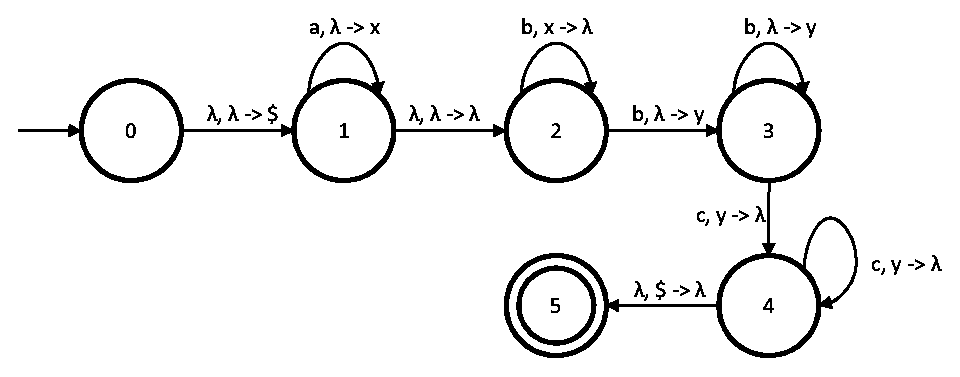
\includegraphics[scale=0.8]{1.eps}
		\caption{PDA of $L = \{ a^n b^{n + m} c^m |n \ge 0,m \ge 1\} $}
	\label{fig:1}
\end{figure}

	
	
	The CFG for $L$ is: \\
	
	$S \rightarrow AB$ 
	
	$A \rightarrow aAb | \lambda$
	
	$B \rightarrow bBc | bc$
	
	\item 
	
		The PDA for $L$ is shown in Figure \ref{fig:2}.
	
	
\begin{figure}[h]
	\centering
		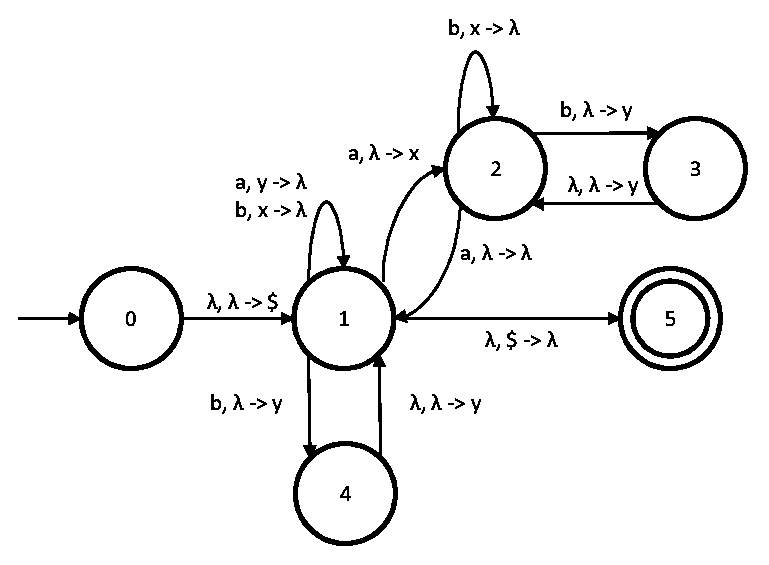
\includegraphics[scale=0.8]{2.eps}
		\caption{PDA of the set of all strings over $\{a, b\}$ with exactly twice as many $a$'s as $b$'s}
	\label{fig:2}
\end{figure}
	
	The CFG for $L$ is: \\
	
	$S \rightarrow aSaSb | aSbSa | bSaSa | \lambda$ 
	
\end{enumerate}
	
	\item Give a context-free grammar in Chomsky Normal Form that generates the following language: 
	\begin{enumerate}
	\item The set of all strings over $\{a, b\}$ with exactly twice as many $a$'s as $b$'s.
	\item $L = \{ w \in (a + b + c)^* |n_a (w) + n_b (w) \ne n_c (w)\}$, where  $n_a (w)$ is the number of $a$'s in $w$.\\	
	\item $L = \{ a^i b^j c^k |i \ne j$  or $j \ne k\} $
	\end{enumerate}
	
	\textbf{Solutions:}\\
	
\begin{enumerate}
	\item The CFG for $L$ is: \\
	
	$S \rightarrow aSaSb | aSbSa | bSaSa | \lambda$ \\
	
	
	The context-free grammar in Chomsky Normal Form for $L$ is:
	
	$S_0 \rightarrow S | \lambda$ 
	
	$A \rightarrow a$
	
	$B \rightarrow b$
	
	$S \rightarrow AA_1 | AA_3 | AA_5 | AA_7 | BB_1 | BB_2 | AA_4|A_4A|BA_8$
	
	$A_1 \rightarrow AA_2$
	
	$A_2 \rightarrow SB$ 
	
	$A_3 \rightarrow SA_4$
	
	$A_4 \rightarrow AB$ 
	
	$A_5 \rightarrow BA_6$
	
	$A_6 \rightarrow SA$
	
	$A_7 \rightarrow SA_8$
	
	$A_8 \rightarrow BA$
	
	$B_1 \rightarrow BA_6$
	
	$B_2 \rightarrow SA_8$
	
	\item The CFG for $L$ is: \\
	
	$S \rightarrow S_1 | S_2 | S_3$
	
	$A \rightarrow aA|a$
	
	$B \rightarrow bB|b$
	
	$C \rightarrow cC|c$
	
	$M_{ac} \rightarrow aM_{ac}c | cM_{ac}a | ac|ca$ 
	
	$M_{bc} \rightarrow bM_{bc}c | cM_{bc}b | bc|cb$ 
	
	$S_1 \rightarrow A S_1 M_{ac}S_1M_{bc}| A S_1 M_{bc}S_1M_{ac} | $ \\ 
	$M_{ac} S_1 A S_1 M_{bc} |M_{ac} S_1 M_{bc} S_1 A| M_{bc} S_1 A S_1 M_{ac} |M_{bc} S_1 M_{ac} S_1 A  $
	
	
	$S_2 \rightarrow B S_2 M_{ac}S_2M_{bc}| B S_2 M_{bc}S_2M_{ac} | $ \\ 
	$M_{ac} S_2 B S_2 M_{bc} |M_{ac} S_2 M_{bc} S_2 B| M_{bc} S_2 B S_2 M_{ac} |M_{bc} S_2 M_{ac} S_2 B  $
	
	$S_3 \rightarrow C S_3 M_{ac}S_3M_{bc}| C S_3 M_{bc}S_3M_{ac} | $ \\ 
	$M_{ac} S_3 C S_3 M_{bc} |M_{ac} S_3 M_{bc} S_3 C| M_{bc} S_3 C S_3 M_{ac} |M_{bc} S_3 M_{ac} S_3 C  $
	
	  The context-free grammar in Chomsky Normal Form for $L$ is: \\
	  
	  $S_0 \rightarrow S$
	  
	  $A \rightarrow a$
	  
	  $B \rightarrow b$
	  	  
	  $C \rightarrow c$
	  
	  $A_a \rightarrow AA_a | a$
	  
	  $B_b \rightarrow BB_b | b$
	  
 	  $C_c \rightarrow CC_c | c$	  
 	  
 	  $M_{ac} \rightarrow AM_{ac2} | CM_{ac3} | AC|CA$ 
 	  
 	  $M_{ac2} = M_{ac}C$
 	  
 	  $M_{ac3} = M_{ac}A$
	
	$M_{bc} \rightarrow BM_{bc2} | CM_{bc3} | BC|CB$ 
	
	$M_{bc2} = M_{bc}C$
 	  
 	  $M_{bc3} = M_{bc}B$
 	  
 	  $S \rightarrow A S_{11} | A S_{14} | M_{ac}S_{17} | M_{ac}S_{19} | M_{bc}S_{112} | M_{bc}S_{115} | $ \\
 	  $B S_{21} | B S_{24} | M_{ac}S_{27} | M_{ac}S_{29} | M_{bc}S_{212} | M_{bc}S_{215}$ \\
 	   $C S_{31} | C S_{34} | M_{ac}S_{37} | M_{ac}S_{39} | M_{bc}S_{312} | M_{bc}S_{315}$ 
 	  
 	  
 	%$S_1 \rightarrow A S_1 M_{ac}S_1M_{bc}| A S_1 M_{bc}S_1M_{ac} | $ \\ 
	%$M_{ac} S_1 A S_1 M_{bc} |M_{ac} S_1 M_{bc} S_1 A| M_{bc} S_1 A S_1 M_{ac} |M_{bc} S_1 M_{ac} S_1 A  $
	
%	$S \rightarrow AS_1|$
	
	$S_1 \rightarrow A S_{11} | A S_{14} | M_{ac}S_{17} | M_{ac}S_{19} | M_{bc}S_{112} | M_{bc}S_{115}$
	
	$S_{11} \rightarrow S_1S_{12}$
	
	$S_{12} \rightarrow M_{ac}S_{13}$
	
	$S_{13} \rightarrow S_1M_{bc}$
	
	$S_{14} \rightarrow S_1S_{15}$
	
	$S_{15} \rightarrow M_{bc}S_{16}$
	
	$S_{16} \rightarrow S_1M_{bc}$
	
	$S_{17} \rightarrow S_1S_{18}$
	
	$S_{18} \rightarrow AS_{13}$
	
	$S_{19} \rightarrow S_1S_{110}$
	
	$S_{110} \rightarrow M_{bc}S_{111}$
	
	$S_{111} \rightarrow S_1A$
	
	$S_{112} \rightarrow S_1S_{113}$
	
	$S_{113} \rightarrow AS_{114}$
	
	$S_{114} \rightarrow S_1M_{ac}$
	
    $S_{115} \rightarrow S_1S_{116}$
    
    $S_{116} \rightarrow M_{ac}S_{111}$
	  
	%$S_2 \rightarrow B S_2 M_{ac}S_2M_{bc}| B S_2 M_{bc}S_2M_{ac} | $ \\ 
	%$M_{ac} S_2 B S_2 M_{bc} |M_{ac} S_2 M_{bc} S_2 B| M_{bc} S_2 B S_2 M_{ac} |M_{bc} S_2 M_{ac} S_2 B  $
		
	$S_2 \rightarrow B S_{21} | B S_{24} | M_{ac}S_{27} | M_{ac}S_{29} | M_{bc}S_{212} | M_{bc}S_{215}$
	
	$S_{21} \rightarrow S_2S_{22}$
	
	$S_{22} \rightarrow M_{ac}S_{23}$
	
	$S_{23} \rightarrow S_2M_{bc}$
	
	$S_{24} \rightarrow S_2S_{25}$
	
	$S_{25} \rightarrow M_{bc}S_{26}$
	
	$S_{26} \rightarrow S_2M_{bc}$
	
	$S_{27} \rightarrow S_2S_{28}$
	
	$S_{28} \rightarrow BS_{23}$
	
	$S_{29} \rightarrow S_2S_{210}$
	
	$S_{210} \rightarrow M_{bc}S_{211}$
	
	$S_{211} \rightarrow S_2B$
	
	$S_{212} \rightarrow S_2S_{213}$
	
	$S_{213} \rightarrow BS_{214}$
	
	$S_{214} \rightarrow S_2M_{ac}$
	
    $S_{215} \rightarrow S_2S_{216}$
    
    $S_{216} \rightarrow M_{ac}S_{211}$
    
% $S_3 \rightarrow C S_3 M_{ac}S_3M_{bc}| C S_3 M_{bc}S_3M_{ac} | $ \\ 

%	$M_{ac} S_3 C S_3 M_{bc} |M_{ac} S_3 M_{bc} S_3 C| M_{bc} S_3 C S_3 M_{ac} |M_{bc} S_3 M_{ac} S_3 C  $
  
  $S_3 \rightarrow C S_{31} | C S_{34} | M_{ac}S_{37} | M_{ac}S_{39} | M_{bc}S_{312} | M_{bc}S_{315}$
	
	$S_{31} \rightarrow S_3S_{32}$
	
	$S_{32} \rightarrow M_{ac}S_{33}$
	
	$S_{33} \rightarrow S_3M_{bc}$
	
	$S_{34} \rightarrow S_3S_{35}$
	
	$S_{35} \rightarrow M_{bc}S_{36}$
	
	$S_{36} \rightarrow S_3M_{bc}$
	
	$S_{37} \rightarrow S_3S_{38}$
	
	$S_{38} \rightarrow CS_{33}$
	
	$S_{39} \rightarrow S_3S_{2310}$
	
	$S_{310} \rightarrow M_{bc}S_{311}$
	
	$S_{311} \rightarrow S_2C$
	
	$S_{312} \rightarrow S_3S_{313}$
	
	$S_{313} \rightarrow CS_{314}$
	
	$S_{314} \rightarrow S_3M_{ac}$
	
    $S_{315} \rightarrow S_3S_{316}$
    
    $S_{316} \rightarrow M_{ac}S_{311}$
	
	\item The CFG for $L$ is: \\
	
	$S \rightarrow A_{i>j}C | B_{i<j}C | AC_{j>k}|AD_{j<k}$
	
	$A \rightarrow aA | \lambda$
	
	$B \rightarrow bB | \lambda$
	
	$C \rightarrow cC | \lambda$
	

	
	$A_{i>j} \rightarrow aA_{i>j}b | aA$
	
	$B_{i<j} \rightarrow aB_{i<j}b | bB$
	
	$C_{j>k} \rightarrow bC_{j>k}c | bB$
	
	$D_{j<k} \rightarrow bD_{j<k}c | cC$\\
	
  The context-free grammar in Chomsky Normal Form for $L$ is:
	
	$S_0 \rightarrow S$ 
	
	$S \rightarrow A_{i>j}C_c | B_{i<j}C_c | A_aC_{j>k}|A_aD_{j<k}$
	
	$A \rightarrow a$
	
	$B \rightarrow b$
	
	$C \rightarrow c$
	
	$A_a \rightarrow AA_a$
	
	$B_b \rightarrow BB_b$
	
	$C_c \rightarrow CC_c$
	
	$A_{i>j} \rightarrow AA_1 | AA_a | A$
	
	$A_1 \rightarrow A_{i>j}B$
	
	$B_{i<j} \rightarrow AB_1 | BB_b | B$
	
		$B_1 \rightarrow B_{i<j}B$
	
	$C_{j>k} \rightarrow BC_1 | BB_b | B$
	
	$C_1 \rightarrow C_{j>k}C$
	
	$D_{j<k} \rightarrow BD_1 | CC_c | C$
	
	$D_1 \rightarrow D_{j<k}C$\\
	
\end{enumerate}
	
\end{enumerate}

\end{document}
